\tikzsetnextfilename{circular_channel}

% Note how the size of all node text has been increased
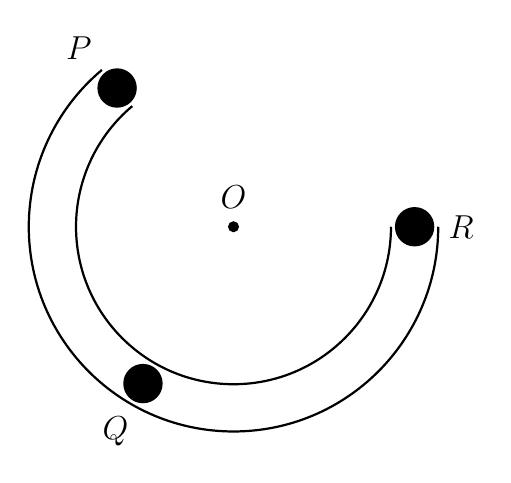
\begin{tikzpicture}[every node/.append style={font=\large}]

    \def\ri{2}
    \def\ro{\ri * 1.3}      % Set outer radius as 30% larger than the inner radius
    \def\ae{-230}           % Angle at end of channel (P)
    \def\aq{-120}           % Angle for point Q

    % Calculate middle of the two radii
    \def\rc{{(\ri + \ro) * 0.5}}        % Note the extra curly braces to encapsulate the arithmetic

    \fill
        (0,0) circle (2pt) node[anchor=south, yshift=3pt] {$O$}
        (\rc, 0) circle (0.25)
        (\ae:\rc) circle (0.25)
        (\aq:\rc) circle (0.25)
    ;

    \draw[thick]
        (\ri,0) arc (0:\ae:\ri)        % Start arc on x-axis and the swing through to -230 degrees with radius \ri
        (\ro,0) node[anchor=west] {$R$} arc (0:\ae:\ro) node[anchor=south east] {$P$}
        (\aq:{(\rc + 0.7)}) node {$Q$}      % Place text a little further ahead than the ball at Q
    ;

\end{tikzpicture}
